% Chapter 1

\chapter{Background Information} % Main chapter title

\label{Chapter1} % For referencing the chapter elsewhere, use \ref{Chapter1}

\lhead{Chapter 1. \emph{Background Information}} % This is for the header on each page - perhaps a shortened title

%----------------------------------------------------------------------------------------

\section{Elderly Issue}
The commonly adopted boundary age for the elderly is 65 years old in
most of the developed counties~\cite{WHO2015}. From the 2010
U.S. census Demographic Profile Data, 13.1\% of the population are
over the age of 65. In Pittsburgh, this ratio is a little higher than
the nationwide statistics (\fref{fig:stat}, which is 13.8\% (42,151),
and 2.4\% (7347) of the population are of age over
85~\cite{censusQuickFact}. By 2030, 72.1 million (19\%) of the U.S
population will be elderly ~\cite{AOA2015}~
\begin{figure}[htbp]
  \centering
  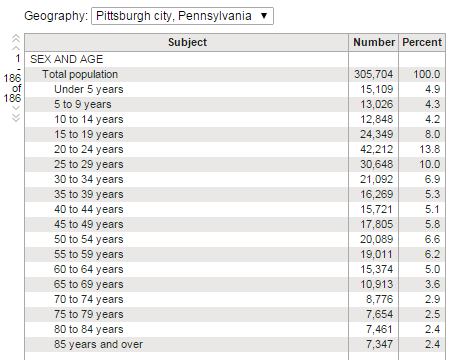
\includegraphics{stat.png}
  \caption[Demographic Information, Pittsburgh]{U.S. census 2010
    Demographic Profile Data (Pittsburgh)~\cite{censusQuickFact}}
  \label{fig:stat}
\end{figure}
%----------------------------------------------------------------------------------------

\par The awareness of the necessity for a senior community center near
Carnegie Mellon University Campus emerged from a previous course
project for Ecological Footprint in Fall 2013 conducted under
instruction of Prof. Hartkopf. In the analysis of the campus
neighborhood, the conflict between the relatively high ratio of senior
population around campus and a lack of proper facilities for senior
citizens was observed .

For imporving quality of life of the neighborhood as a whole,
providing access to safer, more affordable and more environmentally
friendly housing choices for students and faculty members and reducing
the travelling distance of faculty members to provide both more
sustainable and more affordable housing choices, a GIS analysis was
onducted

The series of analysis was conducted with ArcGIS
10.1~\cite{ArcGIS}. First the population density of senior citizen in
the surrounding neighborhood was calculated. The percentage of
population with an age above 65 was adopted as the metric of measuring
the concentration of senior population\cite{WHO2015}. From the
visualization of the senior population distribution, one can observe
that to the south of the campus, there is a large area with a very
high senior population percentage (Figure \ref{fig:seniorPopu}).
\begin{figure}[htbp]
  \centering
  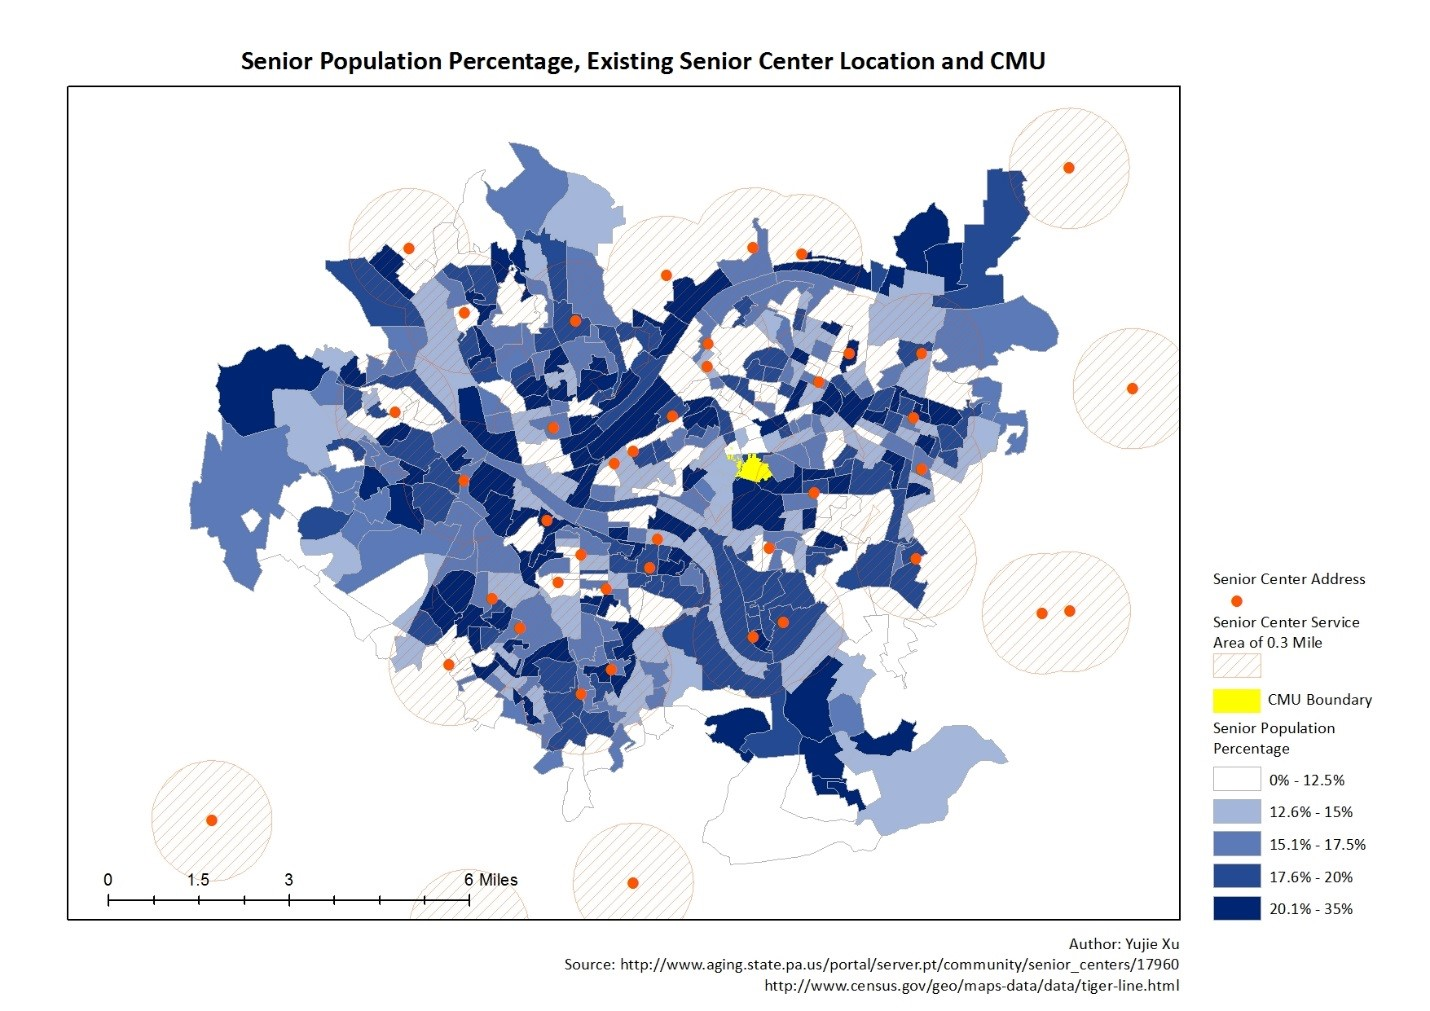
\includegraphics[scale=0.8]{seniorPopu.jpg}
  \rule{35em}{0.5pt}
  \caption[Near-campus Senior Population Density]{Senior Population
    Percentage, Existing Senior Center Location and CMU Campus
    Boundary}
  \label{fig:seniorPopu}
\end{figure}
Then the existing senior centers around Pittsburgh was located on the
map (\tref{tab:seniorCenter}~\cite{aging2013}). See Appendix A for a
list of senior centers located on the map~aref{AppendixA}. A 0.3 mile
service area buffer was created around each existing senior center
facility by applying the approximation analyze. A service area gab
around the campus where no senior center is within a proper walking
distance was identified.

This analysis acts as one of the reasons of the proposal of a senior
community center near CMU campus.

\section{Proposed Site}
\subsection{Surrounding Buildings}
The proposed site of the senior center is to the north of the CMU
campus next to Doherty Apartment across Forbes Ave. It is currently
a parking lot (\fref{fig:siteLocation}). To the north of the proposed
site is the East Campus Parking Garage. To the west of the site lie
the alumni house and the Fraternity/Sorority Quadrangle (\fref{fig:surroundingBd}).
\begin{figure}[htbp]
  \centering
  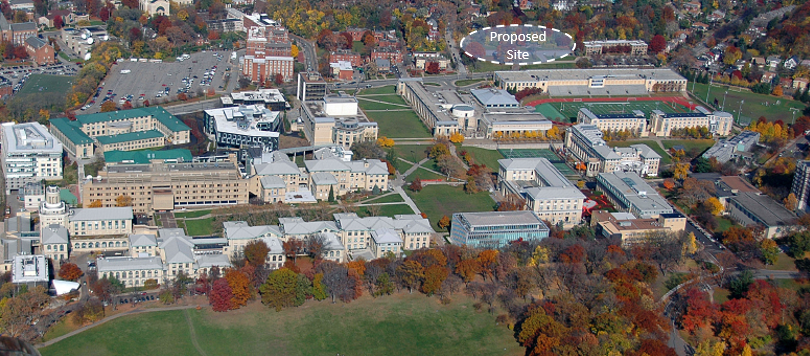
\includegraphics[width=0.7\textwidth]{siteLocation.png}
  \caption[Site Location]{Site Location Ariel View~\cite{masterplan}}
  \label{fig:siteLocation}
\end{figure}
\begin{figure}[htbp]
  \centering
  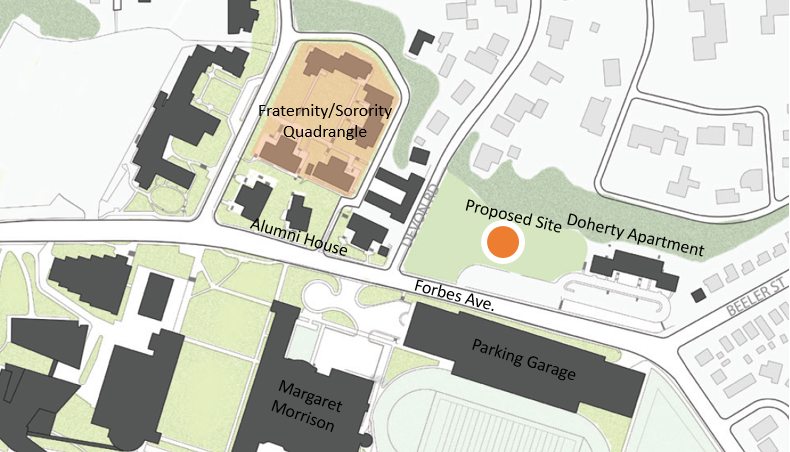
\includegraphics[width=0.7\textwidth]{surroundingBd.png}
  \caption[Surrounding Buildings]{Surrounding
    Buildings~\cite{masterplan}}
  \label{fig:surroundingBd}
\end{figure}
\subsection{Neighborhood Context}
The proposed site of the Senior Community Center is to the north of
Carnegie Mellon University, and is within the boundary of the
Squirrelhill North Neighborhood (\fref{fig:neighborhood}), which
contains the majority portion of the CMU campus. The remaining portion
of the campus is within the North Oakland neighborhood. 

The Squirrehlhill North Neighborhood is in an urban setting. Its
population density is 9713 person per square mile, much higher than
Pittsburgh average (5532). This indicates a less sprawled urban space
pattern and implies a higher chance of creating contact between the
elderly and the society. The neighborhood has a median household
income of \$82,214, over twice of that of the Pittsburgh
(\$35,947). The average household size is 2.1, These features suggest
the community of the proposed site is relatively wealthier and with
small household size. There are 16\% of foreign born residents. This
high ratio of foreign born residents suggest 1) the more urgent need
of a public life than a traditional community with mainly native
residents. The foreign born residents potentially has less social
contact than native residents and thus the community and social life
might be a more important aspect than native residents. 2) The design
of a new Senior Community Center should consider the cultural
difference of senior residents and should provide diversed services
that suits needs of different cultural background.  The area has a
much higher percentage of higher education attainment as a result of
the presence of Carnegie Mellon University.~\cite{neighborhood}
(\tref{tab:neighborStat})
\begin{table}
\begin{tabular}{ p{2in}|c c c c}
\toprule
&Squirrel Hill North&North Oakland&Pittsburgh\\
\midrule
Population Density (people per sq. mile)&9713&14658&5532\\
Median Household Income / \$&82214&40931&35947\\
Median Rent / \$&1123&603&760\\
Percentage of Family Household&45.4&10.9&37.7\\
Percentage of foreign born residents&16&27.5&7.4\\
Housing Price&516844&167225&132337\\
\bottomrule
\end{tabular}
\caption{Neighborhood Statistics}
\label{tab:neighborStat}
\end{table}

Average number of cars or other vehicles in the houses of neighborhood
is 2.2~\cite{neighborhood}. This ratio is high comparing with the
relatively small household size. It implies a less sustainable
traveling pattern. The design impact of the new senior center is that
it should both consider enough parking space, and also the ways to
demonstrate a sustainable travelling method by providing bicycle racks
and car-sharing facilities like a zipcar spot. The zipcar locations
near campus include the East Campus Garage and the parking lot to the
west of Morewood Gardens. 

The neighborhood is older than Pittsburgh average in terms of building
built year. The average estimated housing value (2010) for detached
houses are \$516,844, which is four times that of the Pittsburgh
average of \$132,337. The median rent is \$1,123, which is also a lot
higher than \$603 of Pittsburgh in genera. This rent price is
comparable to that of the renter occupied median housing cost in
Stanford, which indicates the necessity to provide housing for the
newly recruited faculty members (\tref{tab:midHousingcost}). 
\begin{figure}[htbp]
  \centering
  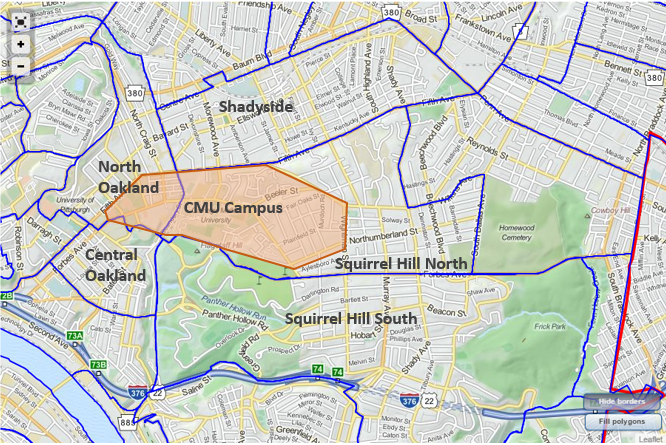
\includegraphics[width=0.7\textwidth]{neighborhood.png}
  \caption[Neighborhood]{Neighborhood Context of Proposed
    Site~\cite{neighborhood}}
  \label{fig:neighborhood}
\end{figure}

\begin{table}
  \begin{tabular}{c | c c c}
    \toprule
    Monthly Housing Cost (Median)	&Occupied	&Owner Occupied	&Renter Occupied\\
    \midrule
    Pittsburgh	&787	&820	&767\\
    Stanford	&1539	&2,933	&1,393\\
    \bottomrule
  \end{tabular}
  \caption{Median Monthly Housing Cost}
  \label{tab:midHousingcost}
\end{table}
\begin{comment}
\end{comment}
\subsection{Historic Aspect}
The site is vacant in 1900, from the history map in 1904, we can see a
brick structured building was present and the building belongs to M.C
Shiller. In 1959, Doherty Apartments is built [8] and has been
functioning ever since. This indicates there are no major historic
context needed to be reflected in the project design nor is there
important historic landmark on the site to be protected
(\fref{fig:history}).
\begin{figure}[htbp]
  \centering
  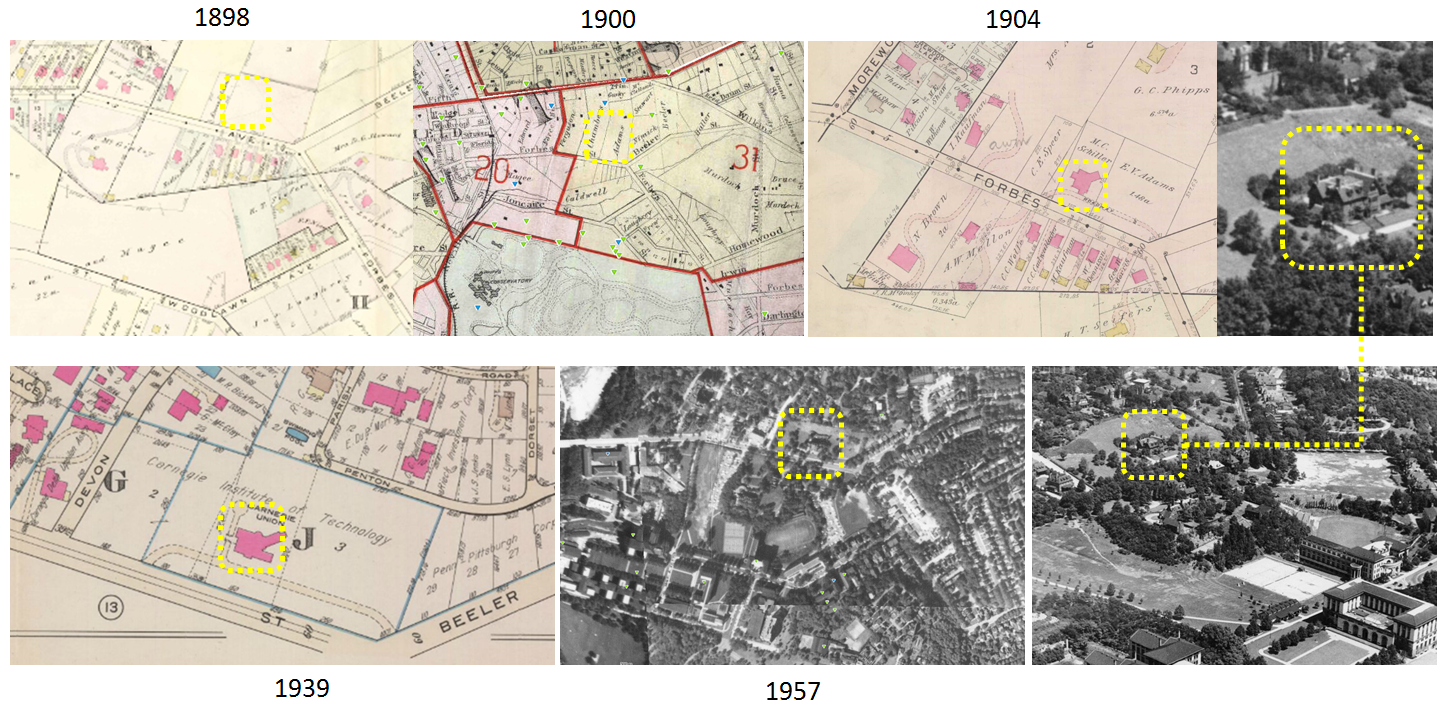
\includegraphics[width=\textwidth]{history.png}
  \caption[History of Site]{The History of the site from 1898 to 1957}
  \label{fig:history}
\end{figure}

\subsection{Physical Condition}
There is an elevation difference between the south and the north of
the proposed site. The north side is about 10m higher than that of the
south. The height difference created a stage for more varied landscape
design opportunities for creating connections between the senior
center, housing for elderly, and the Doherty appartment, housing for
young college students.

\section{Previous Design Conducted}
Ms. Anne-Marie Lubenau has completed a design of a senior center on
this site (~\fref{fig:prevDesign}). The general form of the building
consists of four major clusters: three major living cluster and one
public cluster. Each of the four cluster is easily identified with
the hipped roof above it. The public cluster locate on the
southwestern of the site and the remaining three living clusters
locate on the southeastern, northeaster and northwestern corner of the
building.

The public cluster consists of a public library, a group kitchen, a
lounge on the first floor, a computer cluster, a health suite on the
second floor and some mechanical rooms and storage rooms in the
basement. Each of the living cluster consists of 6 living unit per
floor except the first floor of the northeastern living cluster
consists only 4 living units. There are in total 54 living units in
the building. Between each of the adjacent cluster, there are some
lobby or lounge area. The vertical transportation located in the
center of each of the four cluster. There are 30 parking spot located
in the basement with the entrance on the northeastern corner of the
site.
\begin{figure}[htbp]
  \centering
  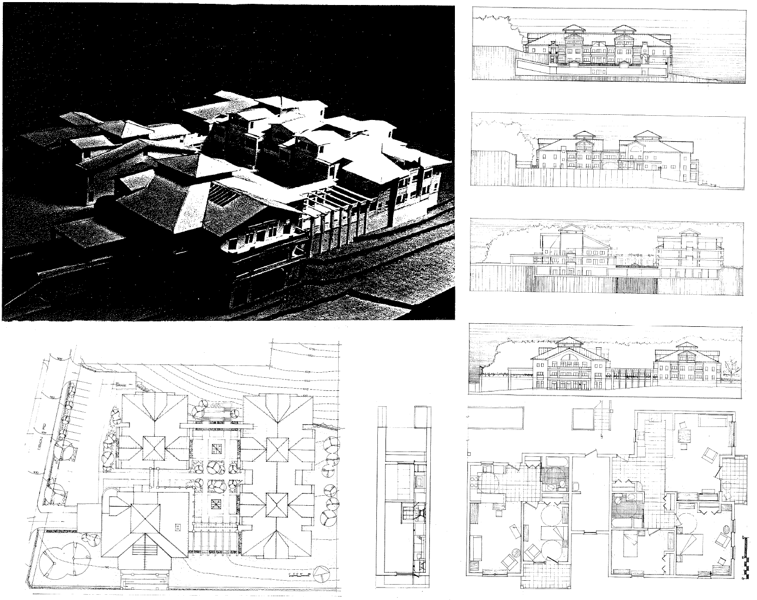
\includegraphics[width=\textwidth]{prevDesign.png}
  \caption[Design by Ms. Lubenau]{Senior Community Center Design by
    Ms. Anna Maria Lubenau}
  \label{fig:prevDesign}
\end{figure}
\section{Climate}
The site located in Pittsburgh, Pennsylvania. It is within the climate
zone 5A, with 5957 Heating Degree Day (HDD) of 65 $\deg F$ and 5009
Cooling Degree Day (CDD) of 74 $\deg$ F. The design heating
temperature is 8 $\deg F$ and design cooling temperature is 86
$\deg F$~\cite{remrate}

From the phschrometric chart, we can see that the dry bulb temperature of the site ranges from 10 to 92 degree F. There is 17\% of the time within the comfort range of 69 to 81 F. 80\% of the time, the temperature is below comfort range and 3\% of the time the temperature is above the comfort range. This indecates the major load for building in this area is heating. 
\begin{figure}[htbp]
  \centering
  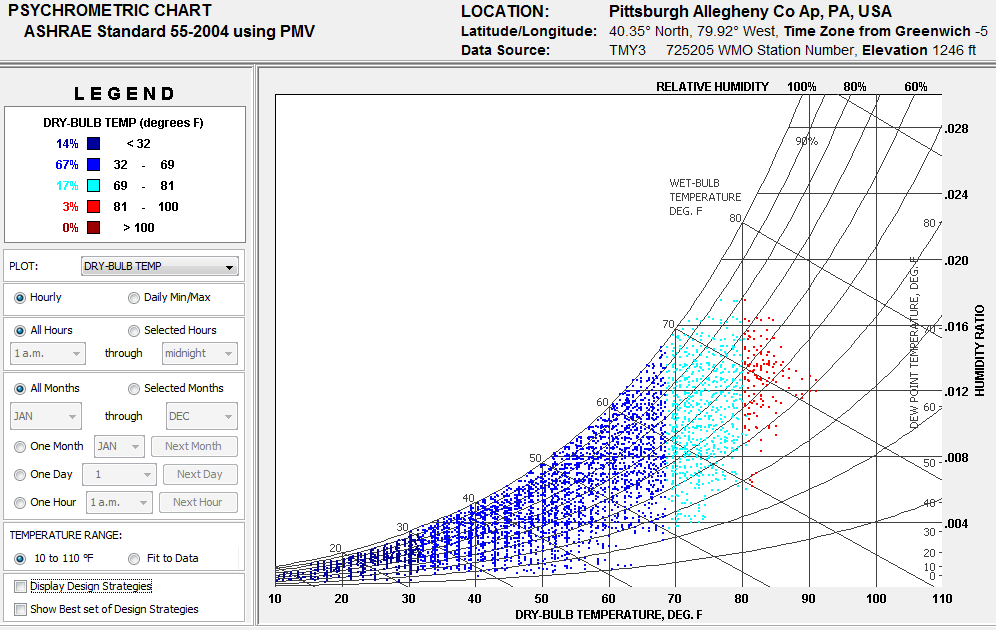
\includegraphics[width=0.7\textwidth]{psChart.png}
  \caption[Phychromatric Chart]{Phychromatric Chart~\cite{climateConsult}}
  \label{fig:psChart}
\end{figure}
From the suggested strategies by Climate Consultant~\cite{climateConsult}, about half of the heating load should be met by heating devices with humidification. The passive strategies for heating season suggested by the software include: ``Internal heat gain'', ``Passive Solar Direct Gain (Low Mass)'' and ``Wind protection''. Internal heat gain is the heat produced by lighting, people activities and equipment operation that warms up the space. This source of heat gain is strongly dependent on the building usage and operation schedules and thus is not a very reliabel strategy. The  ``Passive Solar Direct Gain (Low Mass)'' suggest that providing sun-facing glazing that let in the sunlight can increase the indoor temperature. ``Wind protection'' can pervent the heat loss from infiltration from building entrance. From the wind wheel, we can see in winter (Jan through Feb), the major wind direction is west. The wind with maximum speed comes from southwestern. The design implecation is that the entrance should be arranged so that they are not facing these two directions and have wind protection design in winter.

The passive cooling strageties includes: dehumidification, add sun-shading devices to windows.
\begin{figure}[htbp]
  \centering
  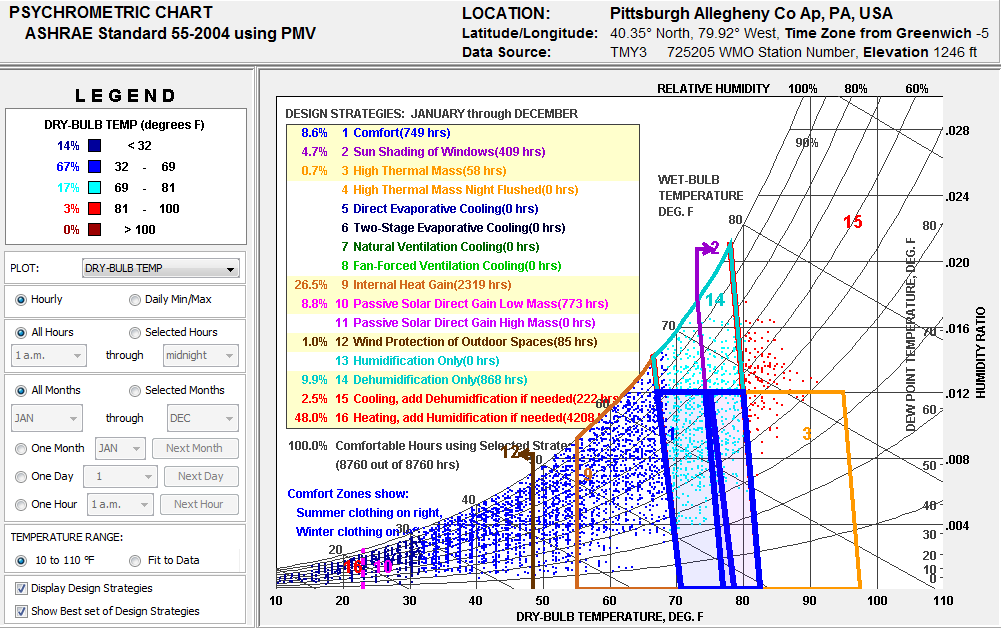
\includegraphics[width=0.7\textwidth]{strategy.png}
  \caption[Phychromatric Chart with Suggested Strategies]{Phychromatric Chart with Suggested Strategies~\cite{climateConsult}}
  \label{fig:strategy}
\end{figure}

\begin{figure}[htbp]
  \centering
  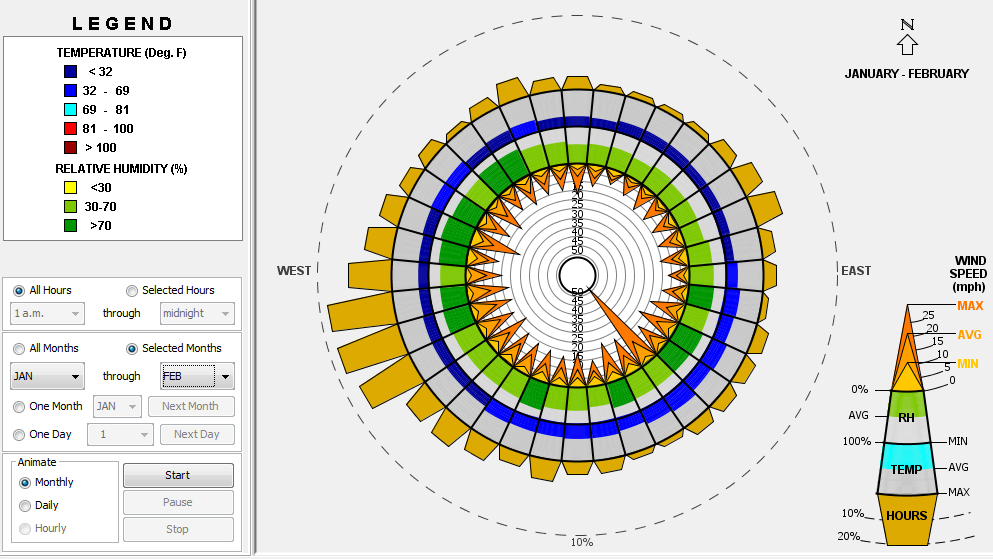
\includegraphics[width=0.7\textwidth]{wind.png}
  \caption[Wind Wheel]{Wind Wheel~\cite{climateConsult}}
  \label{fig:wind}
\end{figure}
\section{Role of the Project}
\subsection{Bridge of Conversation between Different Age Group}
As is addressed by Neyfakh~\cite{Neyfakh2014}, American society is
confronted by severe age segregation, people are hashed into different
``buckets'' of ages groups and their social life is restricted to
their own ``bucket''. No more than 1/4 of the conversation about
``important matters'' happen between the elderly and people younger
than 36; by excluding relatives, the figure dropped to 6\%. Age
segregation ``sow distrust and prejudice between generations, and robs
people of the chance to learn from those younger and older than
them''~\cite{Neyfakh2014}.  The elderly benefit from reading to
children and children or the young people can learn the life knowledge
from the elderly.

One of the major focus of this project is to discuss methods to
establish an inter-generation connection. The role of architecture in
providing good quality of life for the elderly is far more than just
plugging in assisted living facilities and add some space for instant
medical care. It is also about creating chances of meeting new people
and about maintain the link to the society.

\subsubsection{Creating Connections between the Elderly and Children}
One of the elderly friend of Prof. Hartkopf shared his experience of
meeting children in their field trip. Children are the only people
that has the will to touch the elderly apart from the doctors that
give them a shot of drug when they get sick. The age group of elderly
is respected for their rich experiences along the development of
mankind, but is suffering from a segregation as a side-effect of the
development of the modern society.

The presence of a children’s school and the Academy of Lifelong
Learning (\href{http://www.cmu.edu/osher/}{OSHER}) on campus enables
the possibility to create a connection between the life of senior
citizens and the early education of the children in the children's
school.

\subsubsection{Creating Connections between Elderly and Student}
The proposed site is to the east of a student apartment, Doherty
Apartment. The design of a common space on roof level of the senior
center and the bridge from the senior center to the garage might
become a common route for both the elderly and the young colledge
students, which might be able to create interactions between the age
group of the elderly and young students.

Another approach to create the connections between these two age
groups is through volunteering programs where the students can
providing health or activity services for the elderly and the elderly
can also volunteer to participated in some of the study project of
students, especially in aging related areas.

In the discussion with directors in the childrens school, ``Lunchtime
Walking Buddy'' was brought up. It can be an example of how
volunteering opportunities can facilitate the connection between the
two age groups: The path between the proposed site of the senior
community center and the classroom of Lifelong Learning and the
Children's School will bypass the playground. Track walking is an easy
and effective physical exercise for both the elderly and the young. The
problem for the elderly is they might encounter sudden fall while
exercising. The volunteering lunchtime walking will benefit the
elderly by allowing a supervised safer exercise for the elderly and it
will benefit the young by providing them with the chance of
conversation with people of rich life experiences.

Yet another approach is through providing some well designed common
spaces. For example, the common space on the top level of the senior
center could provide a nice study space and the basement will contain
some extra music practicing rooms which might attract young student to
come and use, and thus creating chances for the young and old to meet.

\subsection{Center for Geriatrics (Aging Related) Researches}
There are several geriatrics research groups in or around Carnegie
Mellon University. The creation of such a center near campus can
provide more interactions and hands-on experience with their research
target and thus might assist the development of the related
researches.

\subsubsection{Connections to Quality of Life Technology (QoLT) Center}
The focus of the QoLT center is ``intelligent systems that improve
quality of life for everyone while enabling older adults and people
with disabilities''~\cite{QoLT2014}. One of the promising research
branch of the QoLT center that facilitates the connection to the
Seniro Center is one of the four Testbed Systems: the Home and
Community Health \& Wellness (HCHW), whose goal is described as ``The
goals of the Home and Community Health \& Wellness (HCHW) testbed
systems are to create and evaluate home and community-based solutions
for assessing everyday functional status, providing appropriate
feedback, and assisting rehabilitation in the natural environment for
people with reduced capabilities due to disability or aging.  HCHW
systems will enable more older adults and people with disabilities to
live independently. ''~\cite{HCHW}

The following are some project carried on by the HCHW system:
\begin{itemize}
\item Health Kiosk\\
  The Health Kiosk system allows the elderly to track and record their
  health conditions including ``blood pressure, blood oxygen level,
  handgrip, weight, hearing'' etc. and remotely send the results to
  clinicians without an actual clinical visit. It provides senior
  citizens with easy monitoring and knowledge of their health
  conditions on a regular basis (~\fref{fig:kiosk})~\cite{Kiosk}.
 \begin{figure}[htbp]
   \centering
   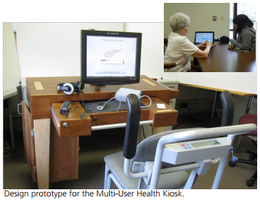
\includegraphics[width=0.5\textwidth]{kiosk.png}
   \caption[Health Kiosk]{Health Kiosk~\cite{Kiosk}}
   \label{fig:kiosk}
\end{figure}
\item Embedded Assessment of Wellness with Smart Home Sensors\\
  The system helps to monitor the abilities of senior citizens in
  performing everyday activities and provides information of the
  degree of physical ability
  declination.~\cite{Lee:2010:EAW:1864431.1864490}
\end{itemize}

\subsection{Community Center for the Elderly and Other Residents}
Although the proposed senior center will contain some amount of living
units to the elderlies with various degree of assistance: from the
active independent elderly, to those need intensive assistance to
those with special needs of assistance (Alzheimer Disease) even the
``end-of-life'' issue. One of the important roles of the center is to
act as a community gathering space dedicated for the surrounding
neighborhood.

\subsection{Demonstration of Advanced Building Technology and System
  Design}
\subsubsection{Urban Agriculture}
Gardening / Horticulture is one of the shared activities of almost all
age groups . It can create food, jobs and a chance of meeting and
mixing of different age groups. Possible approaches of the project on
Urban Agriculture include:
\begin{itemize}
\item Create Roof Gardens on the top floor of the parking garage and
  part of the Senior Community Center

The benifits of using green roof include: reducing stormwater runoff,
protecting roof membrane, reducing heating/cooling load and reducing
urban heat island effect~\cite{Snodgrass2010}.
\item Create Vegetation facade for the Senior Community Center
\end{itemize}
These green space will act as a stage for common activities of
children and elderly to happen; a place to hide from the noise of the
urban jungle; a field to produce food and a classroom for teaching
healthy eating habbits.

\subsubsection{Sustainable / Renewable Energy Source}
\begin{itemize}
\item Solar Energy for electricity: 
  \begin{itemize}
  \item Integration of PV panels and green roofs.
  \item Integration of PV panels and shading devices
  \end{itemize}
\item Geothermal
\item Co-generation system within the building groups
\end{itemize}
\subsubsection{Passive Strategy}
\begin{itemize}
\item Design of building orientation and dimension of space to
  facilitate day-lighting and natural ventilation

Ensure all living units have a south facing window.
\item Rainwater collection and reuse
\item Phase-changing material
\end{itemize}
\subsubsection{Pre-fabrication of Building Components}
\begin{itemize}
\item Using steel or alluminum as the main building structure material.
\item Use a common mode for building design to minimize the number of
  distinct elements.
\end{itemize}
%\subsubsection{Intelligent Building Control System}
\subsubsection{Strategies for Maximizing the Indoor Environment Quality}
\begin{itemize}
\item Water-based heating and cooling system to ensure both the energ performance and the acoustic quality of the indoor environment 
\item Floor-based mechanical system to ensure low pollutant concentration and space flexibility  
\item Transparent space boundary design to allow views to indoor and outdoor activities and to create spatial guidance for the elderly.
\item Installing Personal Environment Module to account for stricter environment requirement from the elderly.
\end{itemize}
\begin{comment}
\section{Benefit for the Elderly}
\subsection{Fighting Age Segregation}
It creates opportunities for fighting "age segregation", a severe problem in the U.S. life style, and facilitates the integration of different age groups.
\subsection{High Quality Continued Education}
\subsection{Adjacency to Art and Culture}
\subsection{Mobility and Green Lifestyle}
\end{comment}
\section{Design Choices and Concerns for Children and Elderly}
Through the discussion with the administrators of the
\href{http://www.psy.cmu.edu/cs/}{children's school} of Carnegie
Mellon University,
Ms. \href{http://www.psy.cmu.edu/cs/people/carver.html}{Sharon
  Carver}, Director of Children's School, and
Ms. \href{http://www.psy.cmu.edu/cs/people/drash.html}{Allison Drash},
the Administrative Coordinator, a lot of insights were acquired about
different approaches about how children and elderly can be related.
\subsection{Integrated Learning Opportunities}
\subsubsection{Dalcroze Eurhythmics}
Music is a common activity shared by all age groups including the elderly and the young children. It is not only a delight for life but also a effective training for brain and physical dexterity development for children and the function maintenance of the elderly. One of such example is the Dalcroze Eurhythmics. It teaches music concepts through body movements.

Eurhythmics is a good candidate for creating common activities between the elderly and the children because: 1) it involves plenty of body movement which can be game-like for children and can be good exercise for the elderly 2) Marta Sanchez Dalcroze Training Center in Carnegie Mellon University has a high quality education in Dalcroze Eurhythmics that offers classes for both the children and the elderly.
\subsubsection{Elderly Reading to Children}
A nursing home in Tulsa, Grace Living Center has a collaboration with the Jenks public school. The facility provids two classrooms for 60 kindergarton students  of grade 1 and 2 and preschool students. The elderly residents in the center can volunteer to become mentors for the children that assists children in both acadamic and social development. Children brought joy in elderly's life, and the elderly provided acadamic improvement for children. The Jenks school found that ``a smaller percentage of students from the GLC have required reading intervention'' in their later studies. One example of the collaborated learning is the ``book buddies'' activities, where children and elderly form groups and read to each other severa times per week. Another example is the ``shared study'', where the elderly and the children work on craft activities together such as making Christmas ornaments, scarecrows etc. There are also comparative course content when the elderly and children share their lifes of ``then and now'' \cite{Morehouse2009}.
\begin{figure}[htbp]
  \centering
  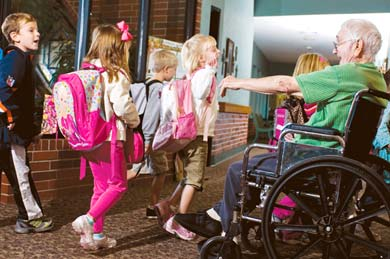
\includegraphics[width=0.5\textwidth]{oldAndYoung.jpg}
  \caption[Ageless Friendship]{Elderly meet School Children at Grace
    Living Center, Tulsa~\cite{Parker2009}}
  \label{fig:oldAndYoung}
\end{figure}
\subsubsection{Horticulture}
The term ``gray and green'', introduced by Wright and
Lund, means the positive effect of introducing
green plants on the process of aging. Gardening reduces stress,
nurtures stewardship~\cite{Wright2000229}. Gardening activities is one
of the common activities that benifit both the children and the
elderly. The ``edible garden'' is mentioned by Tai et al.\ in the book
Designing Outdoor Environments for Children. Edible gardens can let
children experience the whole gardening process from growing to
harvest, promote physical activities and also teach children the
knowledge of healthy eating, which contributes to the battle towards
childhood obesity in the U.S~\cite{Tai2006}, which shortens children's
lifespan expectancy by five years~\cite{Souterbrown2015}. They also mentioned a
type of ``music garden'', where outdoor music instrument are
incorporated in the design of garden environment.

Green space can also act as a healing and conforting power. There are
two major types of such salutogenicly designed gardens: the ``healing
or sensory garden'' that provide passive assist to imporve healthy
conditions. ~\cite{Souterbrown2015}. The ``Healing Gardens'' aims at
providing a quiet and calming space away from urban environment noise,
where ``young and old can escape and emotionally revitalise''. The
``Sensory Garden'' provide a ways to open up the senses of visitors{:
visually, acoustically, variety in scents, tastes and touching
experiences. ``Therapeutic Gardens'' actively conduct healing
operations. There are specific therapeutic gardens for people with
dememtia or mobility problem. A common feature of such therapeutic
gardens is raised bed, which is accessible for people in a wheel
chair.

\subsection{Mobility Issue}
The mobility is a big issue that needs to be seriously dealt with for
the two age groups to meet and have common activities. The elevation
difference, staircases and busy roads can all potentially become
barriers that prevents them from using the path we
designed. Especially for children, in order to reach the proposed site
of the senior center, they have to cross Forbes Ave. According to the
safety requirement, the children need to cross the street with the
presence of traffic lights, so the possible places to cross are either
the crossing at Forbes and Beeler or at Forbes and Morewood. Such
detouring can increase the travel distance and may cause the failure
of establishing such a connection, especially when there are not
enough cleaning and resting facilities as chairs and bathrooms along
the path.

The presence of university center along the path is a great
help. Since the building itself is already a well functioned and
energetic gathering space that provides abundant cleaning and resting
spaces.

One of the desired solution for the detouring and the crossing of
Forbes Ave. is to create a bridge that directly connects the
university center and the senior center. This solution can both
shorten the distance and fulfill the required services along the
path. But from the location of the University Center and the proposed
site, the bridge directly connecting both will be too long to
construct. So instead I propose to connect the parking garage with the
senior center. This bridge may not only act as a safe cross for the
senior people, children as well as the students living in Doherty
Apartment, but also an identification of the entrance to the campus
zone.

The parking garage needs to be retrofitted so that it will not become
an unpleasant spot along the route that only creates noise and exhaust
gas, but a great view. This will be further discussed in the section
of the proposed design of the plants and green space in the senior
center and along the path between senior center and children school.
